\documentclass{beamer}
 
\usepackage[utf8]{inputenc}
\usepackage[english]{babel}
\usepackage{amsmath}
\usepackage{amsfonts}
\usepackage{amssymb}
\usepackage{graphicx} 
\usepackage{latexsym} 
\usepackage{listings}
\usepackage{xcolor}
\usepackage{soul}
\usepackage[T1]{fontenc}
\usepackage{amsthm}
\usepackage{mathtools}
\usepackage{setspace}
\usepackage{array,multirow,makecell}
\usepackage{geometry}
\usepackage{textcomp}
\usepackage{float}
\usepackage{bbold}
\usepackage{wrapfig}
\usepackage{textpos}

\rmfamily

\usetheme{Madrid}
%%\usecolortheme{beaver}



\title{LC 01 Chimie et couleur}
\institute{Université Paul sabatier}
\date{Agrégation 2019}

 
\begin{document}
	
\begin{frame}
	\titlepage
\end{frame}

\addtocounter{framenumber}{-1}
\title{Chimie et couleur}

\begin{frame}
\frametitle{Utilisation des couleurs dans l'histoire : peintures de la grotte de Lascaux}
\begin{figure}[H]
	\centering
		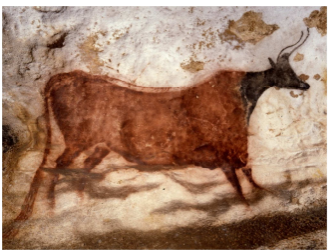
\includegraphics[width=0.46\linewidth]{peinture.png}
		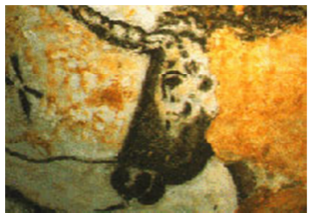
\includegraphics[width=.5\linewidth]{peinture2.png}
\end{figure}
\end{frame}

\begin{frame}
\frametitle{Constitution des couleurs}
\begin{figure}
	\centering 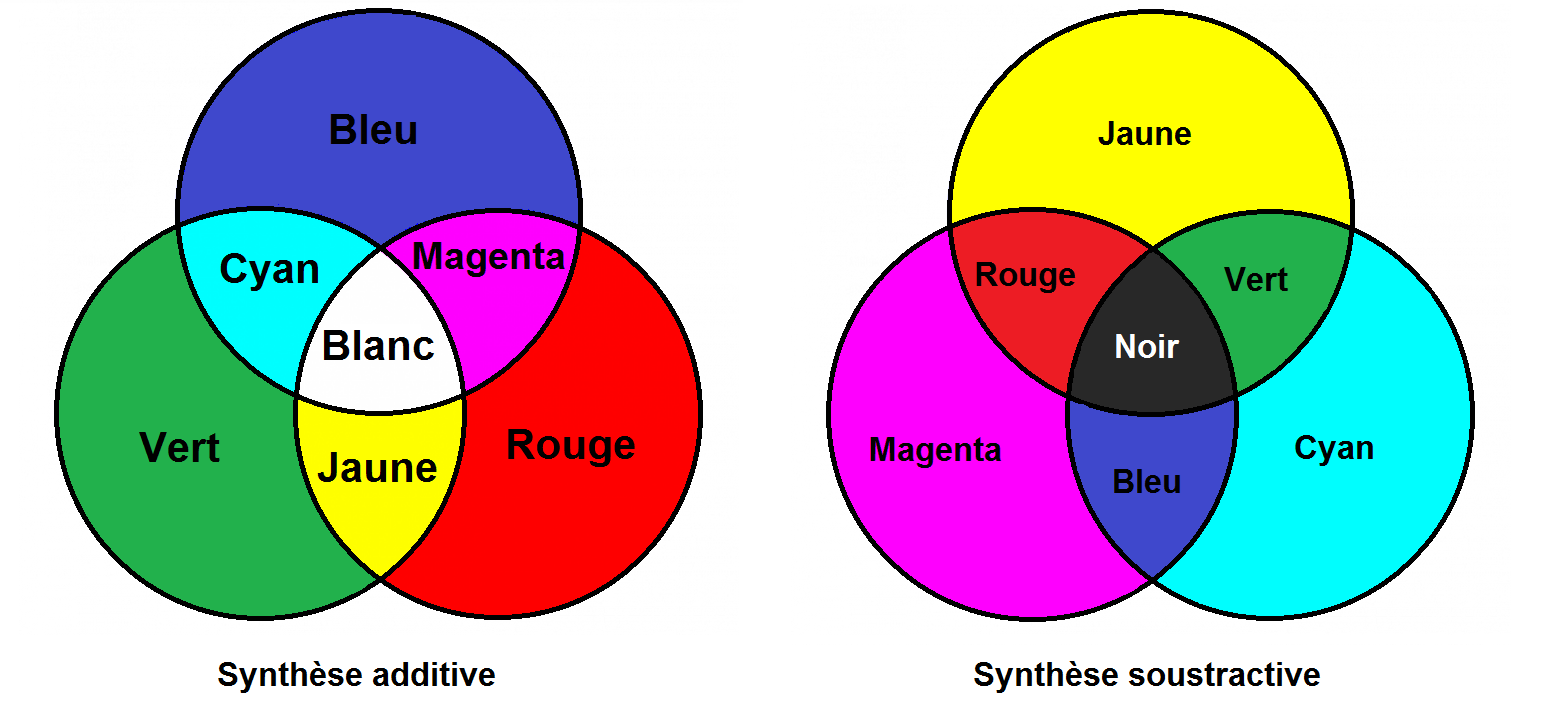
\includegraphics[scale=0.35]{Synthesesoustraddit.jpg}
\end{figure}
\end{frame}

\begin{frame}
\frametitle{La molécule d'indigo}
\begin{figure}[H]
	\centering
	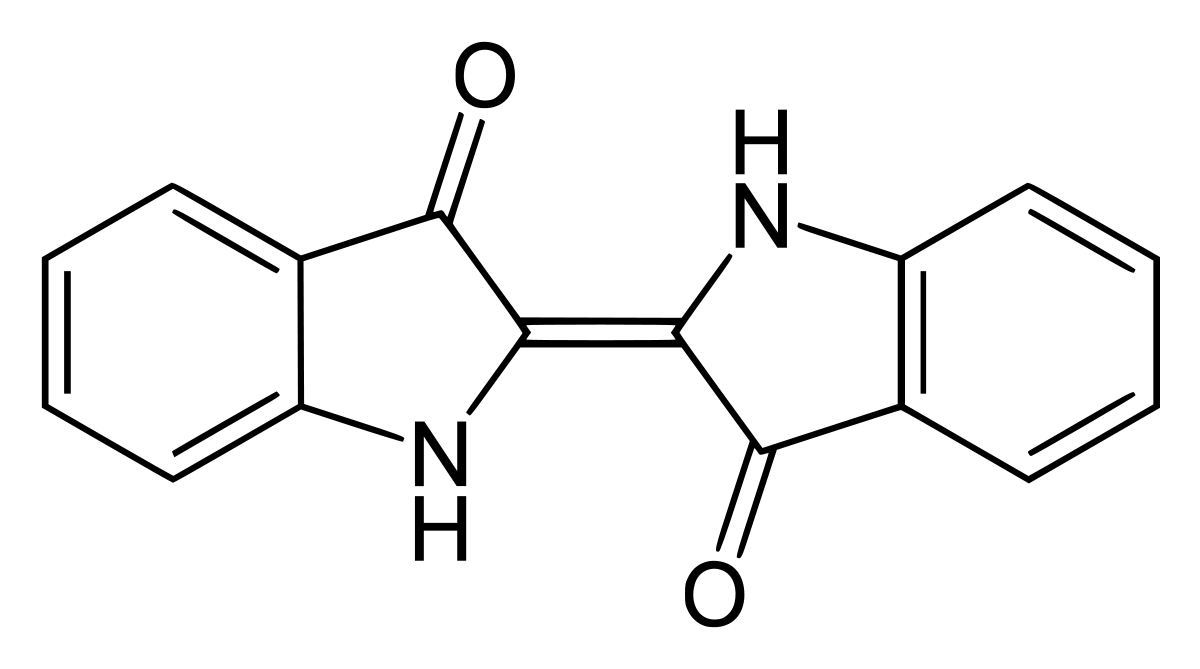
\includegraphics[width =6cm]{Indigomolecule.jpg}
\end{figure}
\end{frame}

\begin{frame}
\frametitle{Liaisons conjuguées et couleur}
\begin{figure}
	\centering
	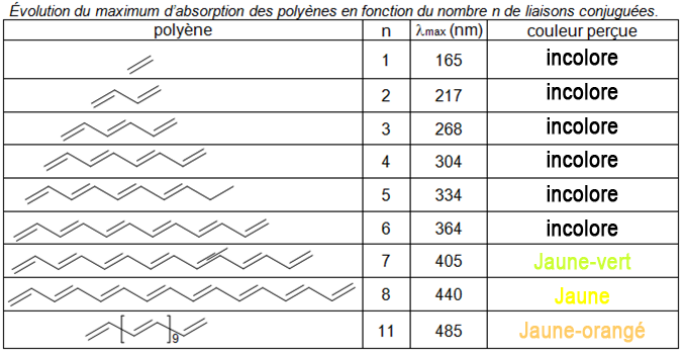
\includegraphics[scale=0.6]{Longonde.jpg}
\end{figure}
\end{frame}

\begin{frame}
\frametitle{Bleu de patenté : spectre d'absorption}
\begin {figure}[H]
\centering
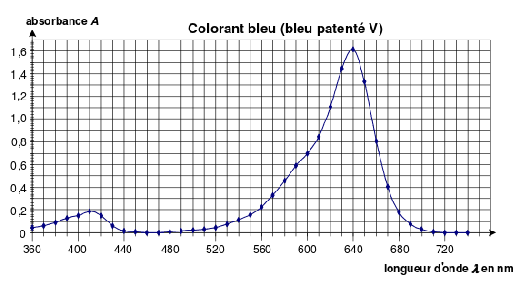
\includegraphics [width =10cm]{E131spectre.jpg}
\end {figure}
\end{frame}

\begin{frame}
\frametitle{Bleu de patenté : molécule}
\begin {figure}[H]
\centering
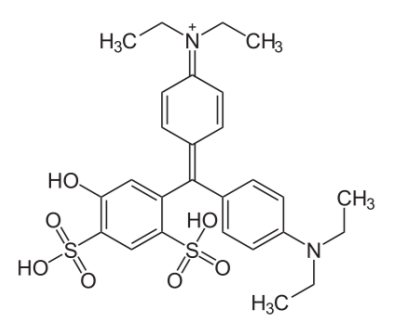
\includegraphics [width =5cm]{E131molecule.jpg}
\end {figure}
\end{frame}

\end{document}